\section{OpenAL}

\emph{OpenAL} (\uv{Open Audio Library}) je softwarový interface k
audio hardwaru. Interface poskytuje několik funkcí, kterými
program modeluje objekty generující ve 3D prostoru a samozřejmě zajišťuje mixování všech zvuků od všech objektů.
Nepodporuje přímo stereo ozvučení, naproti tomu prostě propočítá \emph{streamy} pro potřebný počet kanálů. Nabízí také 
zpracování efektů jako je Doplerův jev, odrazy, překážky,
vysílání a 	dozvuky.

\emph{OpenAL} je implementováno pro většinu platforem.


\subsection{Historie \emph{OpenAL}}

\emph{OpenAL} bylo původně vyvinuto společností \emph{Loki Software} jako
doplněk ke knihovně \emph{OpenGL} asi okolo roku 1998. Dále jej udržuje Creative Technology, která jako první uvolnila hardwarově akcelerovanou \emph{OpenAL}.


\subsection{Stručný popis}

\begin{figure}[hbt]
  \begin{center}
    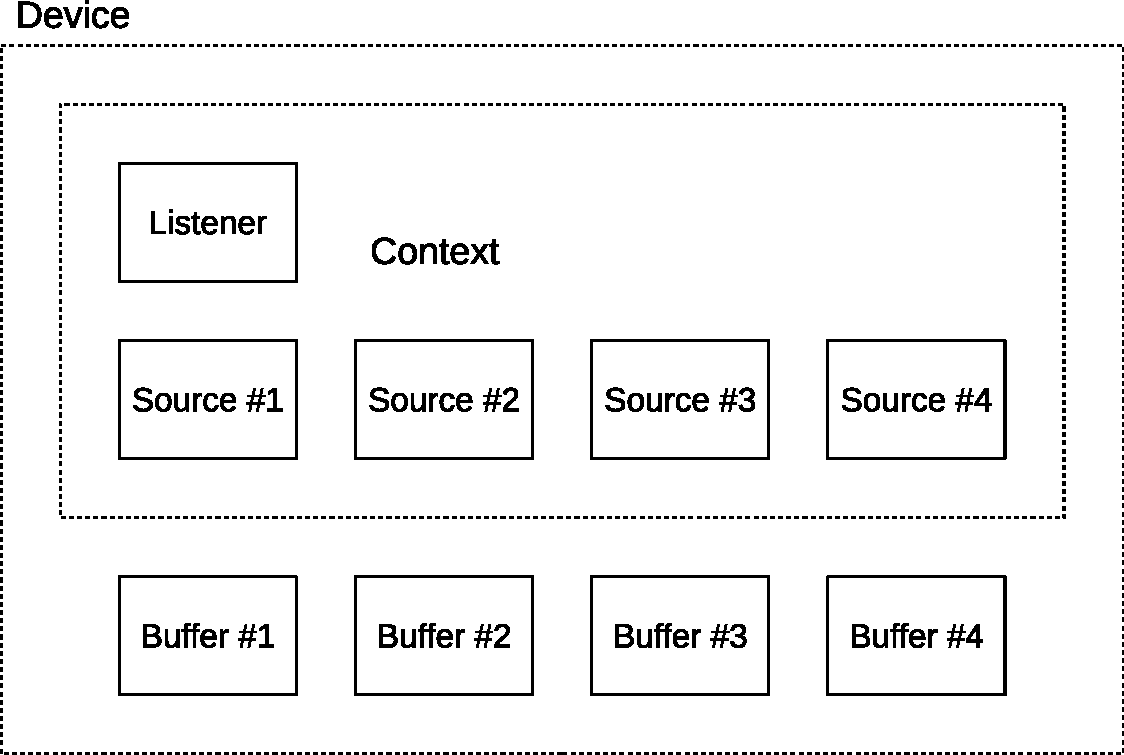
\includegraphics[scale=.6]{obr/openal}
  \end{center}
  \caption{\emph{OpenAL} struktura API}
  \label{obr:openclalassdiagram}
\end{figure}

V \emph{OpenAL} je jeden Posluchač (Listener) který reprezentuje výstup.
Ten je tvořen jedním nebo mnoha, klidně stovkami zvuků od Zdrojů
(Sources). Každý zdroje má kromě zaznamenaného zvuku také přiřazen vzorkovací kmitočet, polohu a vektor rychlosti (pro výpočet Dopplerova efektu). Zdroj přehrává data z jednoho nebo fronty několika bufferů.